\begin{figure}[h]
    \centering
    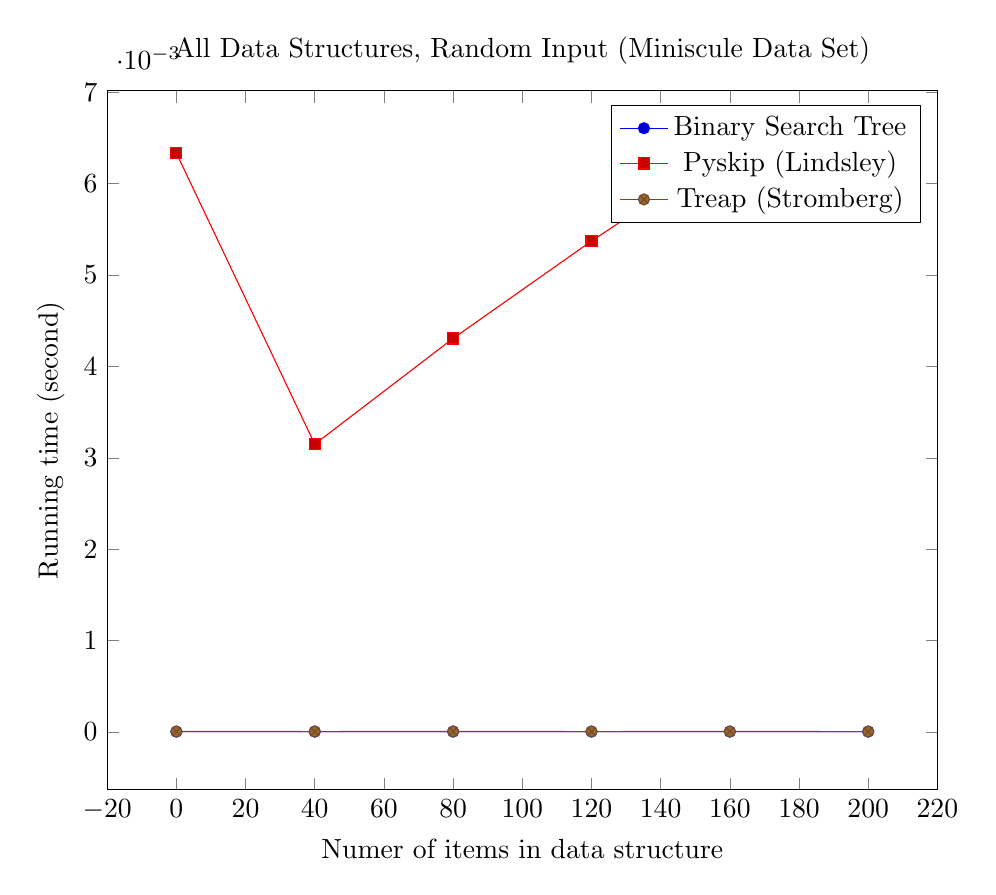
\begin{tikzpicture}
        \begin{axis}[
            xlabel={Numer of items in data structure},
            ylabel={Running time (second)},
            title={All Data Structures, Random Input (Miniscule Data Set)},
            width=\textwidth
        ]
		\addplot coordinates {
			(0, 4.005631978797313e-06)
			(40, 4.457394983924719e-06)
			(80, 4.758570320676468e-06)
			(120, 4.547747584950253e-06)
			(160, 4.698335253326171e-06)
			(200, 4.909157989052212e-06)
		};
		\addplot coordinates {
			(0, 0.006334229329960195)
			(40, 0.0031497217892826777)
			(80, 0.004306777198015288)
			(120, 0.005372094599173316)
			(160, 0.006377357638183012)
			(200, 0.00632073667487365)
		};
		\addplot coordinates {
			(0, 5.391038527946534e-06)
			(40, 5.029628123764951e-06)
			(80, 5.210333325678107e-06)
			(120, 5.029628123764951e-06)
			(160, 5.180215791966703e-06)
			(200, 4.999510590053547e-06)
		};
        \legend{Binary Search Tree, Pyskip (Lindsley), Treap (Stromberg)}
        \end{axis}
    \end{tikzpicture}
    \caption{Average of 10 operations, benchmarked every 40, starting at 0. Median of 11 runs.}
\end{figure}